% !TEX TS-program = pdflatex -shell-escape
% !TEX encoding = UTF-8 Unicode
\documentclass[%draft,
12pt,titlepage,abstracton,DIV=10,BCOR=0.5cm]{scrreprt}
\usepackage[T1]{fontenc}
\usepackage{ucs}
\usepackage[utf8x]{inputenc}
\usepackage[ngerman]{babel}
\usepackage{url,graphicx,xcolor}
%\usepackage{float} % for [H]
\usepackage[pdfstartview=FitH,colorlinks,linkcolor=black,citecolor=darkgray,urlcolor=darkgray,filecolor=darkgray]{hyperref}
%\usepackage{draftwatermark} \SetWatermarkLightness{0}

\bibliographystyle{unsrt}

\usepackage{libertine} %Schriftart Linux-Libertine
\usepackage{courier} % Schriftart für monospaced
\usepackage[activate]{microtype} % Microtype für besseren Zeichensatz

\usepackage{setspace}
\setlength{\parindent}{0pt}
\setlength{\parskip}{9pt}
\onehalfspacing % BA Vorgabe ein-einhalb Zeilenabstand

\usepackage{listings}
\usepackage{pdfpages} % Zum einbinden externer PDF-Dateien

\newcommand{\boppel}[1]{
  \parbox{1cm}{
    \setlength{\unitlength}{1cm}
    \begin{picture}(1,1)(0,0)
      \linethickness{2pt}
      \put(0.5,0.5){\color{cyan}\circle*{1.5}}
      \put(0.5,0.5){\makebox(0,0){\textcolor{white}{\textbf{#1}}}}
    \end{picture}
  }
}

\usepackage[toc,smallcaps]{glossaries}
\renewcommand*{\glstextformat}[1]{\textit{#1}}
\makeglossaries
\makeindex

\title{\infoTitle}
\author{\infoAuthor}
\date{\infoDate}

\setcounter{tocdepth}{1}

\newcommand{\infoTitel}{KSM: Eclipse RCP}
\newcommand{\infoTyp}{Studienarbeit \oldstylenums{2}}
\newcommand{\infoKurs}{Studiengang Informationstechnik}
\newcommand{\infoAutor}{Yves Fischer}
\newcommand{\infoAbgabe}{20. Mai 2011} % Titelseite und Erklärung
\newcommand{\infoBetreuerDH}{Dr. Jörg Wedeck}
\newcommand{\infoKurskuerzel}{\textsc{TIT}2008/NS}

\newglossaryentry{Viewport}{name={Viewport}, description={Begriff aus
    dem Grafikbereich der den Auschnitt eines Bildes, welcher
    dargestellt wird, bezeichnet.}}

\newglossaryentry{Controls}{name={Controls},description={hier Teil einer GUI Anwendung,
oft auch Widget genannt.}}

\newglossaryentry{JDT}{name={JDT},description={\emph{J}ava \emph{D}evelopment \emph{T}ools}}

\newglossaryentry{PDE}{name={PDE},description={Plugin Development
Environment. Oberbegriff für Eclipse Tools zum Entwicklen von Plugins und
RCP-Anwendungen.}}

\newglossaryentry{Classpath}{name={Classpath},description={Der Classpath wird vom Java Classloader benützt um referenzierte Klassen zu finden. Durch spezielle Classloader lässt sich Code innerhalb einer Virtual-Machine separieren.}}

\newglossaryentry{Classloader}{name={Classloader},description={siehe \glstext{Classpath}}}

\newglossaryentry{Memory Leak}{name={Memory Leak},description={Ein Memory Leak ensteht wenn ein Programm (auch indirekt über Bibliotheken) vom Betriebssystem Speicher anfordert (\texttt{*alloc}) und die Referenz auf den zugewiesenen Speicher löscht, daher den Speicher ,,vergisst'' und nicht wieder freigeben kann.}}

\newglossaryentry{KSM/Swing}{name={KSM/Swing},description={Die KSM
Implementierung auf Basis der Java-Swing GUI-Bibliothek.}}

\newglossaryentry{KSM/RCP}{name={KSM/RCP},description={Die KSM
Implementierung als eine Eclipse~RCP Anwendung.}}


\begin{document}
\begin{titlepage}\enlargethispage*{8\baselineskip}
\pagenumbering{roman}
\unitlength1mm
\begin{picture}(0,0)
  \put(26,-15){
\includegraphics[width=10cm]{images/dhbwlogo.png}}
\end{picture}

\vspace{4cm}

\begin{centering}
{
  \fontfamily{\familydefault}
  \fontseries{\seriesdefault}
  %\fontshape{\shapedefault}
  \fontsize{38}{15}
  \selectfont
  {\sc \infoTitel }
}\\
\vspace{1.5cm}
\LARGE{\textsc{\infoTyp}}\\
\vspace{3cm}
\Large{\infoKurs}\\
\normalsize{%
an der Dualen Hochschule Baden-Württemberg\\ Standort Stuttgart Campus Horb\\
von}\\
\vspace{1cm}
\Large{\infoAutor} \\
\vspace{2cm}
\normalsize
Abgabedatum:\\ \infoAbgabe\\
\end{centering}

\vspace{4.0cm}
\begin{tabbing}
MMMMMMMMMMMMMMMMMMMMMMMM                 \= \kill\\
\textbf{Kurs}                            \> \infoKurskuerzel\\
\textbf{Betreuer der Dualen Hochschule}  \> \infoBetreuerDH\\
\end{tabbing}
\begin{flushleft}
\end{flushleft}

\end{titlepage}

{\huge Erklärung}

\vspace{2cm}
Ich habe die Studienarbeit selbständig verfasst und keine anderen als
die angegebenen Quellen und Hilfsmittel benutzt.

Die Arbeit wurde bisher in gleicher oder ähnlicher Form keiner anderen
Prüfungsbehörde vorgelegt und auch nicht veröffentlicht.

\vspace{1cm}

Rheinau, \infoAbgabe

\vspace{1cm}

\_\_\_\_\_\_\_\_\_\_\_\_\_\_\_\_\_\_\_\_\_

\newpage
\renewcommand{\abstractname}{Zusammenfassung}
\begin{abstract}
Im vorangegangen Semester wurde die Portierung der KSM Java/Swing Applikation
auf Eclipse~RCP evaluiert.

In dieser Arbeit sollen konkrete Vorgehensweisen erörtert und der Weg zu
einer Eclipse~RCP basierten KSM Applikation geebnet werden.

\section*{Motivation}
Das GUI von KSM basiert momentan auf Swing bei Verwendung des
NetBeans GUI-\-Designers. Der auf diesem Weg erzeugte Code ist nahezu
unwartbar und auch durch die ständige Weiterentwicklung inkonsistent.

Mithilfe von Eclipse~RCP können dank klarer Strukturen und
Konventionen Verbesserungen im Bereich Wartbarkeit, Erweiterbarkeit
und Usability erzielt werden.

\section*{Problemstellung und Ziele}
Während die vorhergehende Studienenarbeit \cite{fischer10} sich mit der
Einarbeitung in Eclipse~RCP und der grundsätzlichen Möglichkeit der Realisierung
von KSM darin beschäftigte, soll mit dieser Studienarbeit die konkrete Umsetzung
begonnen werden.
\end{abstract}

\renewcommand{\abstractname}{Summary}
\begin{abstract}
The previous assignment evaluated the porting of the KSM Java / Swing
Application to Eclipse-RCP.

This follow-up discuss specific ways  to an Eclipse~RCP based KSM application.

\section*{Motivation} Currently KSM is based on a Java-Swing Graphical User
Interface, developed with the NetBeans GUI-Designer. This GUI-related code is
inconsistent and unmaintainable due to continuos development.

Its possible to gain a better maintainability, expandability and usability by
using Eclipse RCP through clear structures and conventions.

\section*{Tasks and Objectives}
While the foregoing Studienenarbeit elaborates
basic Eclipse-RCP technics and presented a rough-prototype, its now time to
begin with the implementation of specific points of a new KSM Application in
Eclipse-RCP to supersede the Swing-based Application.

The ongoing development will be in close cooperation with students working on
bugfixing and extending the Swing-based KSM, to gain interoperability and quality.
\end{abstract}

\tableofcontents
\newpage\pagenumbering{arabic}

%%%%%%%%%%%%%%%%%%%%%%%%%%%%%%%%%%%%%%%%%%%%%
%%%%%%%%%%%%%%%%%%%%%%%%%%%%%%%%%%%%%%%%%%%%%
\chapter{Einleitung}
Aufbauend auf den Ergebnissen der vorangegangen Studienarbeit gilt es zu
beginnen, mithilfe von Eclipse~RCP ein KSM Werkzeug zu erstellen, welches auf
längere Sicht den die Java/Swing Version ablösen kann.

Für ein KSM auf Basis von Eclipse~RCP sprechen viele Gründe von denen einige
im folgenden kurz erläutert werden:

\textbf{Erweiterbarkeit/Modularität\ } Die Entwicklung von KSM hat viele
verschiedene Versionsstände hervorgebracht die oftmals nicht wieder vereint
werden konnten. Wäre das Grundprojekt modularer aufgebaut gewesen hätten diese
einfacher in ein großes Ganzes integriert werden können.

Zu diesem Zeitpunkt existieren zwei im Grunde gleiche aber getrennte KSM
Entwicklungszweige: KSM und QKSM. Der Ideen und Bugfix Austausch zwischen den
Entwicklern und Projektständen ist durch die strikte Trennung nahezu null.

Wenn zukünftig weitere Anwendungen mit ähnlichen Anwendungsbereich in
Eclipse~RCP entwickelt werden ist es möglich diese mit wenig Aufwand gebündelt
auszuliefern.

\textbf{Vereinfachung\ } Durch Verwendung von Softwarekomponten und Frameworks
aus der Eclipse Plattform kann auf aufwendige, fehleranfällige
Eigenentwicklungen verzichtet werden.

\textbf{Bessere GUI\ } Für Benutzer von Eclipse wird das Arbeiten mit Workspaces
und Projekten beim Umgang mit KSM bereits vertraut sein. Alle anderen werden mit
einer intuitiven, Standard- --- weniger individuell-kreativen --- Oberfläche
konfrontiert.

\textbf{Lizenzmanagement\ } KSM soll in naher Zukunft öffentlich verfügbar
sein, QKSM nicht. Wäre QKSM ein Zusatzmodul (Bundle, Plugin) für KSM, dann
würde lediglich eine zusätzliche Datei einem Open-Source KSM QKSM Fähigkeiten
verleihen.

\textbf{Deployment/Update\ } Eclipse verfügt über ausgereifte Mechanismen zur
Softwareverteilung und Aktualisierung. Über eine Update-Site könnten Benutzer
über das Internet Ihre KSM-Installation modular Ihren Bedürfnissen anpassen und
aktualisieren.

\textbf{Web Anwendungen\ } Mithilfe von RAP (Rich Ajax Platform) lassen sich
RCP Anwendungen ins Web portieren.

Nicht zuletzt soll die wertvolle Erfahrung des Umgangs mit einer ,,open source,
robust, full-featured, commercial-quality, industry platform for the development
of highly integrated tools and rich client application'' erwähnt werden.

\vspace{1cm}

Diese Studienarbeit wird die Vorteile der Nutzung der Eclipse Plattform nur zum
Bruchteil auskosten. Nicht zu vergessen ist, dass es auch Hindernisse gibt auf
die im Kapitel \ref{chapter:rcpprogrammierung} ab Seite
\pageref{chapter:rcpprogrammierung} eingegangen wird.

Zu Beginn wird die Entwicklung eines Datenformat für die Computerdarstellung von
Kybernetischen System-Modellen besprochen. Kapitel
\ref{chapter:weiterentwicklung} beschreibt Veränderungen gegenüber dem Prototyp
aus der vorhergehenden Arbeit.

In Kapitel \ref{chapter:rcpprogrammierung} wird auf das Erlernen des Umgangs und
die Arbeit mit Eclipse~RCP/PDE besprochen. Kapitel \ref{chapter:ausblick}
wird die Ergebnisse dieser Arbeit kurz zusammenfassen und zur möglichen
Weiterentwicklung Stellung nehmen.

%%%%%%%%%%%%%%%%%%%%%%%%%%%%%%%%%%%%%%%%%%%%%
%%%%%%%%%%%%%%%%%%%%%%%%%%%%%%%%%%%%%%%%%%%%%
\chapter{Datenformat und Datenmodell}
In der Studienarbeit 1 wurde mit einem vereinfachten Datenmodell gearbeitet.

Da zukünftig sowohl KSM/Swing als auch /RCP die gleichen Daten verarbeiten
können sollten, liegt es nahe, dass das Format in dem die Daten persistent im
Dateisystem abgelegt sind, vereinheitlicht werden sollte.

Im folgenden wird ausgeführt warum das aktuelle Datenformat in KSM/Swing nicht
geeignet ist und wie ein neues entwickelt wurde.

\par
\begingroup
\leftskip=1.5cm % ggf. verstellen
\noindent In Anhang \ref{chapter:doku-datamodel} ist die vollständige Dokumentation des
neuen Datenformat zu finden, dessen Entwicklung in diesem Kapitel beschrieben
wird.
\par
\endgroup

\section{Istzustand}
In der Evaluation von RCP wurde ein einfaches Datenformat eingeführt, indem die
Model-Objekte einfach mittels leicht annotierten JAXB serialisiert wurden
\cite[S. 22f]{fischer10}: {\small
\begin{verbatim}
<?xml version="1.0" encoding="UTF-8" standalone="yes"?>
<diagram>
    <connections>
        <connection>
             <source>1c862df6-80e5-445b-a41c-ed677973abfb</source>
             <target>e36a0368-d8f6-40a2-bd29-375352045da8</target>
        </connection>
    </connections>
    <nodes name="Node 01">
        <id>1c862df6-80e5-445b-a41c-ed677973abfb</id>
        <location>
             <x>128</x>
             <y>90</y>
        </location>
        <nodeProperties/>
    </nodes>
    <nodes name="Node 11">
        <id>e36a0368-d8f6-40a2-bd29-375352045da8</id>
        <location>
              <x>531</x>
              <y>104</y>
        </location>
        <nodeProperties/>
    </nodes>
</diagram>
\end{verbatim}
}

In der aktuellen KSM/Swing Applikation wird ebenfalls ein auf XML-basierendes
Datenformat verwendet.

Abbildung \ref{fig:ksmswing-diagramm} zeigt ein einfaches KSM-Diagramm in
KSM/Swing. Listing \ref{ksmswingdata} gibt sehr stark gekürzt das bei der
Speicherung erzeugte XML wieder.

\begin{figure}[ht!]
  \centering
  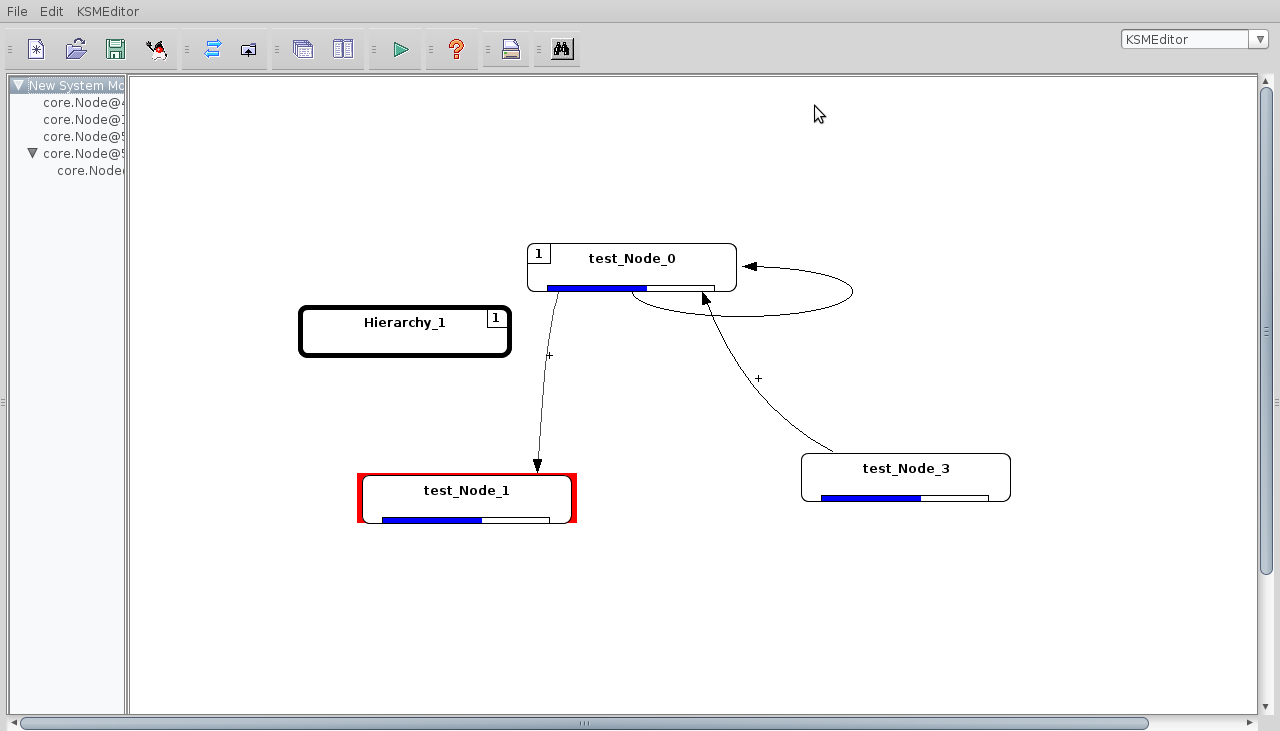
\includegraphics[width=\textwidth]{images/ksm-swing-screenshot.png}
  \caption{KSM/Swing Applikation bei der Anzeige der Daten aus Listing
  \ref{ksmswingdata}}
  \label{fig:ksmswing-diagramm}
\end{figure}

\lstinputlisting[language=XML,basicstyle=\ttfamily\scriptsize,
	caption={Datenformat aus KSM/Swing Applikation Stand
	22.02.2011}]{files/ksm-example.xml}\label{ksmswingdata}

Für das KSM/Swing Datenformat existiert ein XML-Schema in der Ausarbeitung der
Studienarbeit von Friedhelm Wolf \cite{wolf05} in Anhang 4. Es wurde aber in den
folgenden Studienarbeiten nicht mehr weiter gepflegt und ist daher vermutlich
nicht mehr gültig.

Darüberhinaus existierte keine saubere Dokumentation dieses Datenformates. Die
Bedeutung der abgelegten Werte muss aus dem Quelltext von KSM/Swing
interpretiert werden - was nicht immer einfach ist.

Weiterhin scheinen die Konventionen beim Entwurf dieses Formates (oder
,,Schema'') eher beliebig gewesen zu sein.
Dies fällt als erstes auf bei der Benennung der der Eigenschaftsnamen (Tags), wo
\texttt{CamelCase} (,,Microsoft Stil''), \texttt{javaStilArt} und
\texttt{underline\_stil} wild gemischt werden. Die Benamung verwendet teils
einen Typ-Prefix (\texttt{sIconPath}), teils auch nicht.

Die Ein- und Ausgabe erfolgt in KSM/Swing mithilfe der Java-Bibliothek
\textit{com.\-machine\-dialog}. Von Seiten der Projektbetreuung wurde geäußert,
dass es gewünscht ist diese alte Bibliothek nicht mehr weiter zu verwenden. Zu den
genauen Gründen sei auf die Studienarbeit\,\oldstylenums{1} von Tobias Dreher
verwiesen \cite[S. 24]{dreher10}.

Die fehlende Dokumentation und der anscheinend unstrukturierte Entwurf sprachen
ebenfalls gegen die Weiterverwendung dieses Datenformates.
In Sicht zur Zukunft ist das Format ungeignet, weil es nicht erlaubt, dass
zusätzliche Eigenschaften rückwärtskompatibel abgebildet werden.

Weiterhin ist es ist nicht (mehr) durch ein XML-Schema gestützt und es wurde im
Laufe der Entwicklung mehrmals beliebig verändert. Es ist nicht dokumentiert und
der Parser in KSM/Swing Programm ist in einem schlechten, mit der GUI
verknüpften Zustand.

\section{Entwicklung eines neuen Datenformat}
Wie an diesen beiden Beispielen zu sehen ist, bietet das XML-Format aus der
Studienarbeit~1 nicht das Ausdrucksvermögen des KSM/Swing Format. Letzteres ist
jedoch ungeeignet zur Nutzung in einer neuen KSM RCP-Applikation.

Daher lag es nahe ein Format zu entwerfen, welches sowohl von KSM/Swing mithilfe
einer sauberen neuen Import/Export Infrastruktur als auch in der RCP-Anwendung
genutzt werden kann. Es wurde hierbei ein Ansatz gewählt der sowohl Knoten,
Gruppen von Knoten (auch bekannt als ,,Hirarchien'') als auch gerichtete
Verbindungen zu einem anderen Knoten abbilden kann. Alle drei Objekte können
durch Eigenschaften dynamisch, nicht schema-gebunden mit Informationen
angereichert werden.

\par \begingroup \leftskip=1.5cm % ggf. verstellen
\noindent

Die Implementierung des Exports in das neue Datenformat in \textbf{KSM/Swing}
wurde von Tobias Dreher vorgenommen. Siehe dazu seine Studienarbeit
\cite{dreher11}. \par

\endgroup

Zu festen Standardisierung wurde ein XML-Schema erstellt, woraus wiederum
mittels des XML-Schema-Compiler (xjc) von JAXB Java-Klassen erzeugt werden, die
mit weiteren, handgeschrieben Klassen eine Bibliothek zur Abbildung von
KSM-Diagrammen im Speicher sowie Funktionen zum Laden und Speichern bietet (Abb.
\ref{fig:class-diagram-xmlschema}). Diese kann sowohl von KSM/RCP als auch
beliebigen Java-Anwendungen verwendet werden.

\begin{figure}[ht!]
  \centering
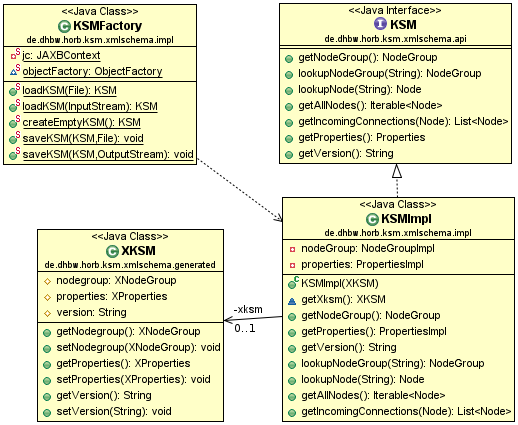
\includegraphics[width=0.8\textwidth]{images/class-diagram-xmlschema.PNG}
\caption{Klassendiagramm XML-Datenmodell Bibliothek, Ausschnitt KSM
Model-Klasse}
\label{fig:class-diagram-xmlschema}
\end{figure}

Die Datenmodell Bibliothek (Projektname:
\texttt{ksm-model}) ist als Eclipse-Project angelegt, kann jedoch auch nur mit
Apache-Ant verwaltet werden (ist somit Netbeans kompatibel). Das Projektverzeichnis enthält weiterhin
umfassende Unit-Tests, teils im Beaviour-Driven Stil mithilfe der Bibliothek
\textit{mockito}.

Listing \ref{listing:example} zeigt valide Beispieldaten zu dem im Anhang ab
Seite \pageref{listing:schema} hinterlegten, neuen XML-Schema.

\lstinputlisting[language=XML,basicstyle=\ttfamily\scriptsize,
	caption={KSM Daten im neuen Datenformat (example-1.xml)}
	]{files/example-1.xml}\label{listing:example}


Weitere Dokumentation zum Format und der Bibliothek finden sich im Anhang ab
Seite \pageref{chapter:doku-datamodel}.


%%%%%%%%%%%%%%%%%%%%%%%%%%%%%%%%%%%%%%%%%%%%%
%%%%%%%%%%%%%%%%%%%%%%%%%%%%%%%%%%%%%%%%%%%%%
\chapter{Weiterentwicklung Programmfunktionalität und
Modularisierung}\label{chapter:weiterentwicklung}

Das KSM/RCP Projekt besteht aus folgenden Komponenten:
\begin{description}
  \item[\texttt{de.\-dhbw.\-horb.\-ksm.\-core}] Plugin
  Project, Kernfunktionalität:
  \begin{itemize}
    \item RCP-Anwendung; Einstiegspunkt
  	\item Editor auf Basis von GEF (Figures, EditParts, Policies, Commands)
  	\item Projekttyp (\textit{Nature}), Projektwizard, Outline und Navigator
  	\item KSM-Properties-Description Extension-Point
  \end{itemize}
  \item[\texttt{de.\-dhbw.\-horb.\-ksm.\-qksm}] Fragment Project von
  \texttt{.core}, enthält nur eine Demo für den Property Extension-Point.
  \item[\texttt{de.\-dhbw.\-horb.\-ksm.\-simulator}] Plugin Project, Enthält eine Demo der
  Live-Verknüpfung des im Editor dargestellten Modells mit einem Chart auf
  Basis von SWTChart.
  \item[\texttt{de.\-dhbw.\-horb.\-ksm.\-tableeditor}] Plugin Project, enthält
  einen Prototyp zum Editieren von Knoteneigenschaften in Tabellenform.
  \item[\texttt{ksm-model}]
  Java-Project/Apache Ant, Datenmodell:
  \begin{itemize}
    \item XML-Schema des Datenformat.
    \item Java Library auf Basis von JAXB.
    \item Dokumentation des Datenformat.
  \end{itemize}
  \item[\texttt{de.\-dhbw.\-horb.\-ksm.\-model}] Plugin Project welches
  \texttt{ksm-model} als OSGi-Bundle zur Verfügung stellt. Muss nach
  Aktualisierung von \texttt{ksm-model} ebenfalls aktualisiert werden.
\end{description}

Das \texttt{\ldots qksm}-Projekt ist als Eclipse-Projekt vom Typ
,,Plugin-Fragment'' abgelegt. Das bedeutet, es hängt direkt vom KSM-Core Plugin
als Host-Plugin ab und ist kein eigenständiges (OSGi-)Bundle. Es wird wird beim
Start mit dem Host-Plugin vereinigt. Diese vorgehensweise eignet sich um ein
Plugin ohne es zu verändern nachträglich um Features, wie z.B.
Internationalisierung oder plattformabhängigen Code, zu erweitern.

Ein Fragment Projekt unterscheidet sich von einem Plugin Projekt in weiteren
Punkten. Da es kein eigenständiges Bundle ist, besitzt es keine
Activator-Klasse. Die Datei zur Beschreibung der Extensions heißt
\texttt{fragment.xml} anstatt \texttt{plugin.xml}. In
\texttt{META-INF/MANIFEST.MF} wird daher kein Activator deklariert - jedoch mit
\texttt{Frag\-ment-Host} das zu erweiternde Plugin.

Das \texttt{\ldots model} Projekt wurde durch den Eclipse Assistenten ,,Plug-In
from existing JAR'' erstellt. Es enthält die \texttt{.class} Dateien aus dem JAR
das im Projekt \texttt{ksm-model} durch ant erzeugt wird. Die zukünftige
Aktualisierung kann einfach dadurch erfolgen, dass die Class-Files von Hand in
das \texttt{\ldots model} Projekt kopiert werden. Dadurch dass man auf diesem
Weg das \texttt{ksm-model} Projekt als OSGi Bundle zur Verfügung hat können
KSM/RCP-erweiternde Plugin dieses einbinden. Alternativ wäre es möglich gewesen
die \texttt{.jar}-Datei aus \texttt{ksm-model} in das \texttt{\ldots
core}-Projekt einzubinden und von dort aus zu exportieren. Damit müsste jedoch
mit jeder Änderung in \texttt{ksm-model} das \texttt{\ldots core}-Plugin
,,angefasst'' werden.

Das \texttt{ksm-model} Projekt wurde aus Rücksicht auf die
nicht-Eclipse Entwicklung frei von Eclipse-Abhängigkeiten gehalten und nicht
gleich als OSGi-Bundle implementiert.


\section{Die RCP Applikation \texttt{ksm.\-core}}
Eine grafische Eclipse~RCP Anwendung verfügt immer über ein zentrales Plugin als
Einstiegspunkt in die Ausführung. Diese implementiert das Interface
\texttt{IApplication} und registriert sich auf den Extension-Point
\texttt{org.\-eclipse.\-core.\-runtime.\-app\-licat\-ions}. Die
\texttt{IApplication}-Klasse erzeugt den \texttt{Work\-be\-nch\-Advisor} welcher
das grundlegende Aussehen mithilfe von Perspektiven und anhand einem
\texttt{Work\-bench\-Window\-Advisor} steuert \cite{vogelrcp}.

Im \texttt{\ldots ksm.core} Plugin ist die gesamte KSM-Editierfunktionalität
enthalten. Dazu gehört der GEF-basierte Editor, das Outline und die
Projektansicht.



\subsection{Der grafische Editor und das Datenmodell}
\begin{figure}[ht]
\centering
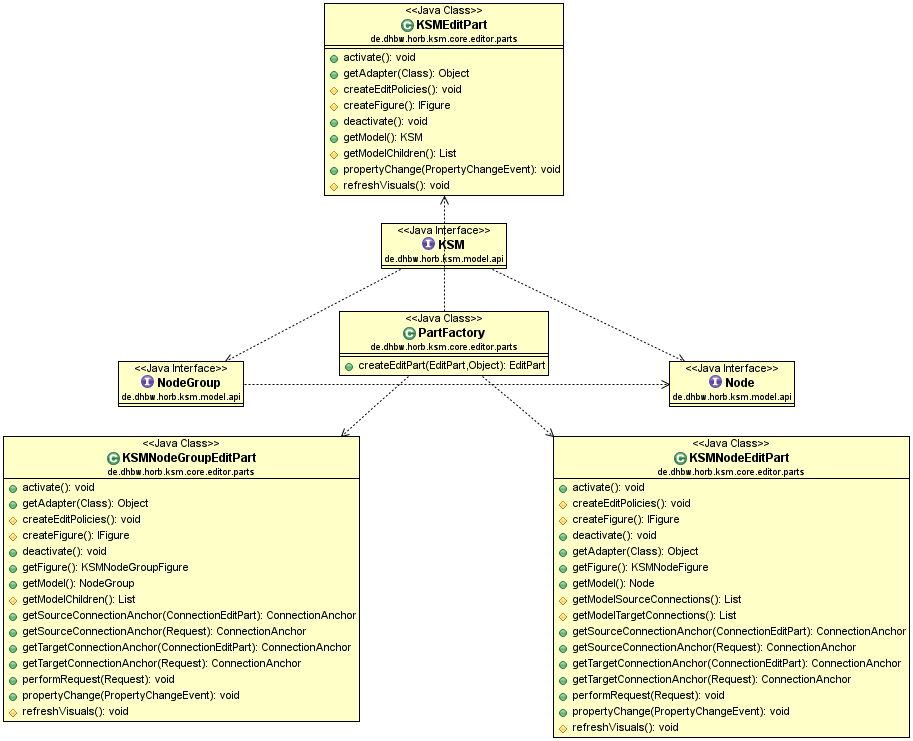
\includegraphics[width=\textwidth]{images/model.PNG}
\caption{Model und View von KSM/NodeGroup/Node}
\label{fig:model}
\end{figure}

Der mit dem Graphical Editing Framework (GEF) umgesetzte Editor ist teil des
\texttt{\ldots ksm.\-core} Plugin-Projekt. GEF geht von einem existierenden
Datenmodell aus welches hier durch das Plugin-Project \texttt{\ldots ksm.model}
anstelle von \texttt{ksm-model} zur Verfügung gestellt wird.

Bei der ,,Initialisierung'' eines GEF-Editors wird dem Editor eine Factory
zugewiesen die für die Objekte/verschiedenen Typen des Datenmodells
GEF-EditParts erzeugen kann
(\texttt{Diagram\-Editor\-\#configureGraphicalViewer}, Abb. \ref{fig:model})
\cite{gef1}.

Anschliessend wird das Datenmodell zugewiesen
(\texttt{DiagramEditor\-\#initialize\-Graph\-ical\-Viewer}). Der GEF-Editor ruft
nun mit dem ,,Parent''-Objekt des Datenmodells die \texttt{Part\-Factory} auf
und erhält das entsprechende EditPart. Der weitere Abstieg in der Hirarchie des
Datenmodells geschieht durch den Aufruf von
\texttt{Graphical\-Edit\-Part\-\#getModel\-Children()} welcher eine Liste von
Kind-Elementen des jeweiligen Elementes ergibt. So liefert bspw. die KSMEditPart
hier alle NodeGroup- und Node-Elemente aus der Root-NodeGroup des Datenmodels.


\begin{figure}[ht]
\centering
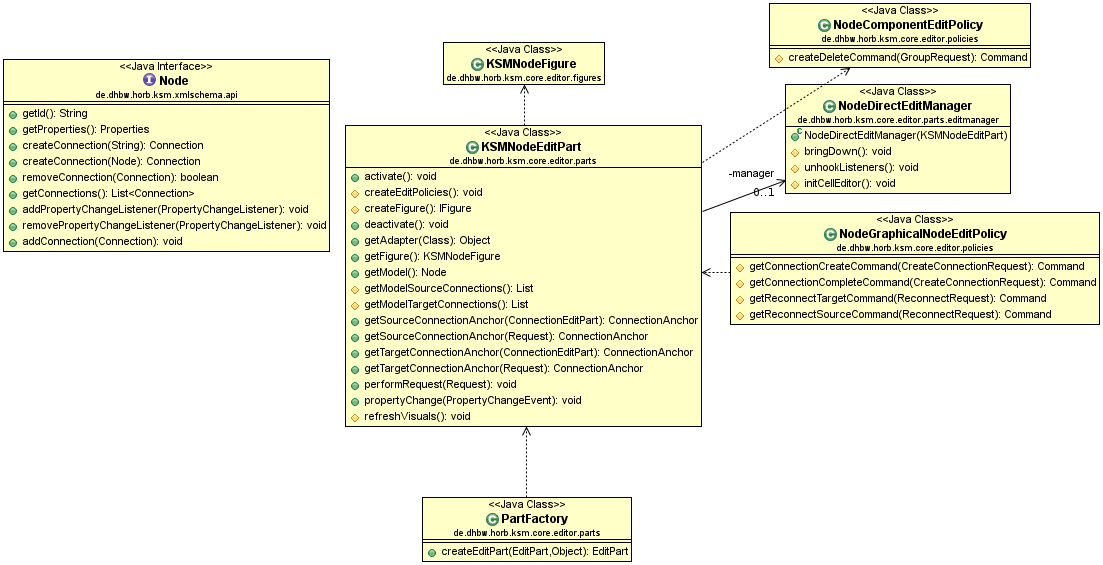
\includegraphics[width=\textwidth]{images/node-edit-and-figure.PNG}
\caption{Model, View und Controller des Node-Typ (von Rechts nach Links)}
\label{fig:node-edit-and-figure}
\end{figure}

Das GEF Programmiermodel ist dem \textit{Model-View-Controller} Pattern
angelehnt. Abbildung \ref{fig:node-edit-and-figure} zeigt am Beispiel des KSM-Typ aus dem Datenmodell
die Zugehörigkeit der Klassen zu Model, View und Controller.

Die Edit-Policies erfüllen die Rolle des Controllers indem sie definieren, was
passieren soll wenn bestimmte Umstände eintreten. U.a. falls der Benutzer
angefordert hat das Element zu löschen (z.B. durch Drücken der Entfernen Taste)
oder einen ,,Direct-Edit'' durch einen langsamen Doppel-Klick angefordert hat.

\subsection{Commands}

\begin{figure}[ht]
\centering
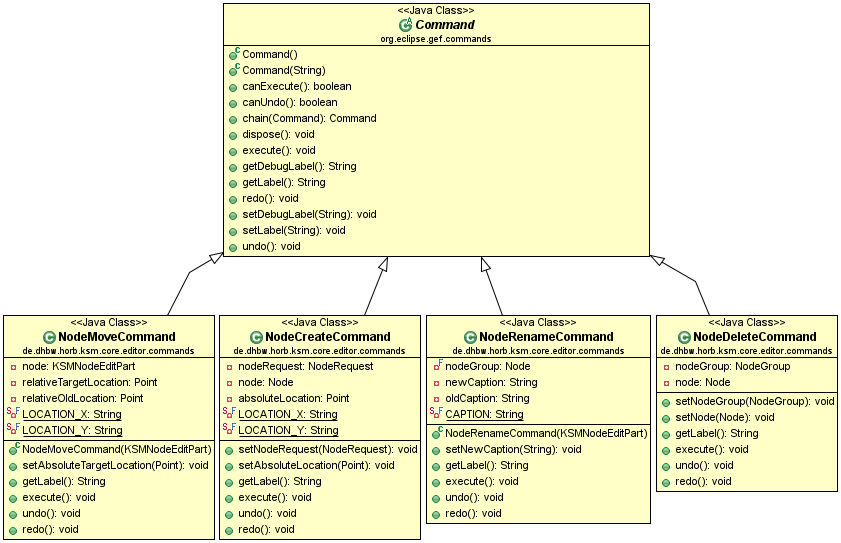
\includegraphics[width=0.9\textwidth]{images/commands.PNG}
\caption{Command Basisklasse und Commands betrefft dem \texttt{Node}-Typ}
\label{fig:commands}
\end{figure}

Alle Manipulationen des Datenmodells werden durch sogenannte \texttt{Commands}
beschrieben. Abbildung \ref{fig:commands} zeigt die Basisklasse und abgeleitete
Klassen die Manipulationen des \texttt{Node}-Typ beschreiben.

Commands implementieren jeweils die Durchführung der Manipulation als auch das
rückgängig Machen. Durch GEF werden die Commands bei Anwendung auf einem Stack
abgelegt wodurch das klassische Undo/Redo ermöglicht wird.

Dieses Pattern verhindert weiterhin, dass das Datenmodell an beliebigen
Code-Stellen manipuliert wird trägt so zur allgemeinen Wartbarkeit bei.



%zooming redbook 4.2.4
% übersicht der commits mit verbesserten commit-messages

% fragment project versus bundle



% Properties
% http://www.eclipse.org/articles/Article-Properties-View/properties-view.html
% vogella: extension points



\section{Simulation}
Das ,,Simulation'' Project \texttt{\ldots ksm.simulator} zeigt als Prototyp wie
es möglich ist, Daten die im Editor bearbeitet werden live mit einem Chart
auszuwerten.

Der Chart ist als View implementiert. Die View besitzt mehrere
Zustände/Ansichten für alle KSM-Editoren die geöffnet sind und es wird immer die
zum aktuell fokussierten Editor passende dargestellt.

Für den Linechart wird die Bibliothek SWT-Chart verwendet die dem Projekt
beigelegt ist. Sie wird im OSGi-Manifest angegeben:
{\small\begin{verbatim}
...
Bundle-ClassPath: lib/org.swtchart_0.7.0.v20110128.jar,
 lib/org.swtchart.ext_0.7.0.v20110128.jar,
 .
\end{verbatim}}

Der Prototyp der Simulationsdarstellung trägt lediglich die X- und Y-Position
des KSM-Nodes auf die Y-Achse auf und die KSM-Node-Beschriftung auf die X-Achse.

\begin{figure}[ht!]
\centering
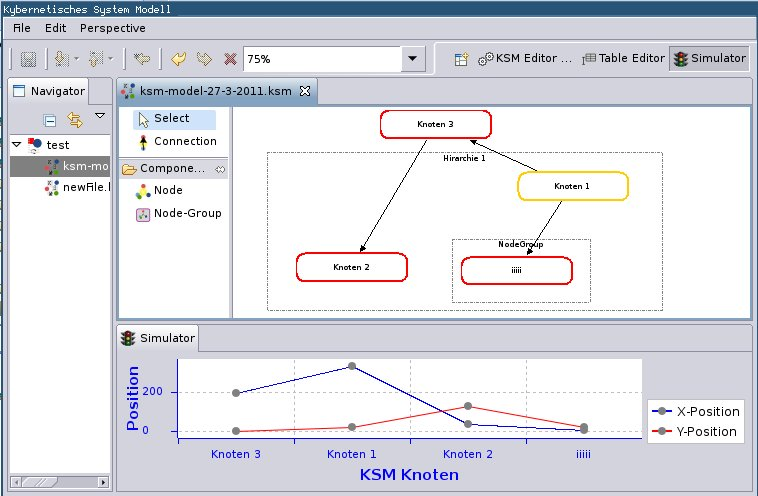
\includegraphics[width=0.8\textwidth]{images/eclipse-simulator.jpg}
\caption{Simulator Prototyp}
\label{fig:eclipse-simulator}
\end{figure}


\section{Property Editor}
Damit ein Model für die Standard Eclipse-Properties-View nötigen Informationen
bereitstellt muss eine \texttt{Prop\-erty\-Source} bereitgestellt werden. Dies geschieht im
einfachen Fall indem die Model-Klasse \texttt{IProp\-erty\-Source\-Provider}
implementiert wird.

Ist dies nicht der Fall fragt die Properties-View das \texttt{EditPart} über
\texttt{getAdapter\-(IProp\-erty\-Source\-Provider.class)} nach einem Objekt,
das die Properties des Model beschreibt. Dieser Ansatz wurde gewählt, da die
Klassen des Models nicht angepasst werden konnten. Dies ist in einer
Designschwäche der Model-Bibliothek begründet. Es ist noch nicht möglich eigene,
abgeleitete Klassen für das Model zu verwenden.

Es wurden daher die Klassen \texttt{\ldots core.\-editor.\-model.\-property.*}
als PropertySourceProvider für \texttt{Node} und \texttt{NodeGroup} eingeführt.
Abbildung \ref{fig:ext-property-descriptors} zeigt als UML-Klassendiagramm die
Klassen zur Verwaltung der Properties.

\begin{figure}[mt]
\centering
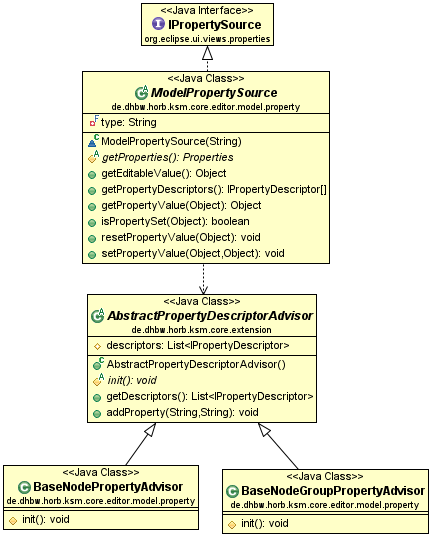
\includegraphics[width=0.5\textwidth]{images/ext-property-descriptors.PNG}
\caption{Klassen des Extension Point für Property Deskriptoren}
\label{fig:ext-property-descriptors}
\end{figure}

\begin{figure}[ht]
\centering
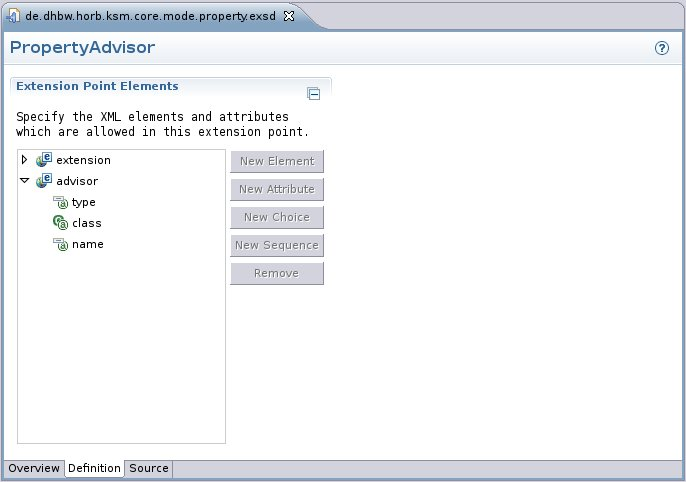
\includegraphics[width=0.7\textwidth]{images/eclipse-property-declaration-extensionpoint.jpg}
\caption{Deklaration des Extension-Point für Property-Advisors}
\label{fig:property-declaration-extensionpoint}
\end{figure}

\begin{figure}[ht!]
\centering
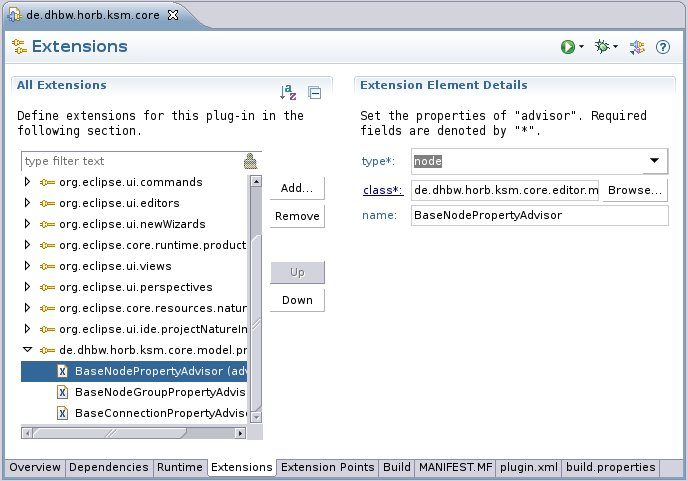
\includegraphics[width=0.7\textwidth]{images/eclipse-property-usage-extensionpoint.jpg}
\caption{Benutzung des Extension-Point für Property-Advisors}
\label{fig:eclipse-property-usage-extensionpoint}
\end{figure}

Für jedes Model-Objekt meldet das entsprechende EditPart eine Instanz von
\texttt{Model\-Property\-Source}. Das Attribut \texttt{type} ist dabei je nach
Model eines von \texttt{ksm, node\-group, node, con\-nection}.
Anhand dieses Typs wird in der Extension\-Registry nachgeschlagen ob für den
Extension\-Point \texttt{de.\-dhbw.\-horb.\-ksm.\-core.\-model.\-property}
Extensions registriert wurden.

Extensions sehen so aus, dass eine von
\texttt{Abstract\-Property\-Descriptor\-Advisor} abgeleitete Klasse (im
Beispiel sind schon BaseNode[Group]PropertyAdvisor dargestellt, die die
Manipulation der grundlegenden Eigenschaften Farbe und Beschriftung erlauben)
angegeben wird die Descriptoren für Eigenschaften des Model-Objekt erstellt.

Abbildung \ref{fig:property-declaration-extensionpoint} zeigt wie der Extension
Point deklariert wurde. Das gezeigte GUI ist eine Maske für eine XML-Datei die
im Prinzip ein XML-Schema für das XML ist mit dem der Extension-Point von
Client-Plugins konfiguriert wird. Auf diesen Extension-Point können beliebig
viele ,,advisor'' Elemente angelegt werden, die auf eine von
\texttt{Abstract\-Property\-Descriptor\-Advisor} abgeleitete Klasse zeigen und
ein Attribut \texttt{type} haben (Abb.
\ref{fig:eclipse-property-usage-extensionpoint}).


\section{Table-Editor}
Der Table-Editor ,,besteht aus sechs Reitermenüs. Diese besitzen folgende
Funktionalitäten: [Editoren für] ,Edge Values' – Kanteneigenschaften [..]
,Node Values' – Knoteneigenschaften'' (Studienarbeit Christian Riess \cite[S.
24]{riess03}).

Abbildung \ref{fig:table-editor} zeigt den Table-Editor der im Rahmen dieser
Studienarbeit prototypisch entworfen wurde.

\begin{figure}[ht]
\centering
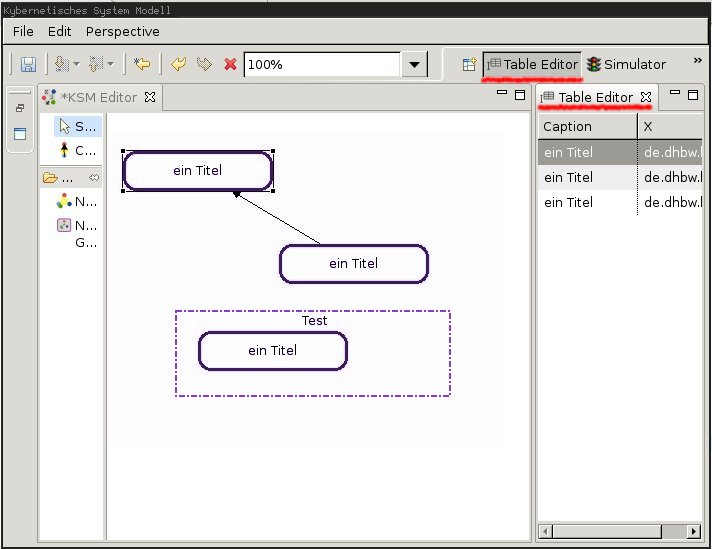
\includegraphics[width=0.8\textwidth]{images/table-editor.jpg}
\caption{Prototyp eines Table-Editor}
\label{fig:table-editor}
\end{figure}

Rot markiert ist die neue View des ,,Table-Editor''. Sie wird durch den Aufruf
der Table-Editor Perspektive aktiviert (Button ist ebenfalls rot markiert).

Bei der View handelt es sich um eine von abgeleitete Klasse
\texttt{PageBookView}. Sie instanziert für jeden offenen Editor einen
Table-Editor. Es wird jeweils der zu dem fokussierten Diagramm-Editor passende
Table-Editor angezeigt. Die Implentierung folgt dabei dem Eclipse-Standard wie
er auch in Outline verwendet wird.

Änderungen am Diagramm übernimmt der Table-Editor einfacherweise nicht indem er
auf alle Node/NodeGroup Objekte Listener registriert, sondern er beobachtet den
Command-Stack des Editors. Dies funktioniert nur solange alle weiteren
Änderungen am Modell Command-Objekte im Diagramm-Editor Command-Stack erzeugen.

Der Table-Editor nutzt im Prototyp noch keine Undo-/Redo-Funktionalität sondern
arbeitet ,,dreckig'' direkt am Datenmodell.

%%%%%%%%%%%%%%%%%%%%%%%%%%%%%%%%%%%%%%%%
%%%%%%%%%%%%%%%%%%%%%%%%%%%%%%%%%%%%%%%%
%%%%%%%%%%%%%%%%%%%%%%%%%%%%%%%%%%%%%%%%
\chapter{Eclipse~RCP Programmierung}\label{chapter:rcpprogrammierung}
Dieses Kapitel soll zukünftigen Entwickler einige Hinweise zum schnellen Start
geben. Dazu soll die in dieser Arbeit verwendete Arbeitsumgebung vorgestellt und
die dabei gewonnenen Erfahrungen bei der Einarbeitung und Nutzung mitgeteilt
werden.

Weiterhin werden Vorschläge zur stärken Integration von Eclipse-Tools in das
Studium aus der Sicht eines Studenten vorgestellt.

Es bei dieser Studienarbeit mit dem Eclipse \oldstylenums{3}.6/Helios Package
,,for RCP and RAP Developers'' gearbeitet.

\section{Hilfsmittel}
Zu Beginn der Studienarbeit I verfügte ich über Basiskentnisse der Eclipse
Java Development Tools (JDT). Das Thema Eclipse~RCP wurde im Studium nicht
angesprochen und daher war meine primäre Aufgabe einen Einstieg in das Thema
RCP-Entwicklung zu finden.

Zum Kennenlernen von Eclipse ist der Besuch einer Eclipse Demo~Camp
Veranstaltung empfehlenswert. Dort werden neue, auf Eclipse aufbauende
Technologien vorgestellt. Informationen darüber finden sich im Eclipse Wiki
\cite{eclipse:wiki}. Weitere aktuelle Informationen aus dem Eclipse Umfeld
finden sich in Blogs die im Eclipse Planet aggregiert werden
(\url{http://planeteclipse.org/}).

Weiterhin ist auch einige der Literatur in Buchform, die im Literaturverzeichnis
dieser Arbeit verlinkt ist, sehr hilfreich. Grundsätzlich findet man jedoch die
meisten Informationen in RCP-Beispielapplikationen, formloser Dokumentation und
im Eclipse-(Online-)Hilfesystem. Auch sollte man zur RCP-Entwicklung die Quellen
von RCP installiert haben, sodass man bei jeder Gelegenheit nahtlos in den
Quellcode von RCP wechseln kann. Die API-Dokumentation der RCP und auch GEF
Klassen ist meist sehr hilfreich.

Zum Einstieg ist das RCP Tutorial von Lars Vogel empfehlenswert \cite{vogelrcp}.
Zu den Grundlagen von GEF sind die Folien eines EclipseCon Tutorials interessant
\cite{gefslides}. Tiefergehende jedoch teils veraltete Informationen bietet
das IBM RedBook zu GEF \cite{gefredbook}.

Einen allgemeinen Überblick und guten Enstieg in die Eclipse Plugin Entwicklung
findet sich in der Seminararbeit im Kurs Software-Engineering
2011/\textsc{TIT2008} von Felix Kienzle \cite{kienzle11}.

Da Eclipse~RCP kein monolithisches Produkt ist sondern sich aus einzelnen
Komponenten zusammensetzt findet man auch Informationen jenseits von RCP.
Beispielsweise zu OSGi\cite{bartlett}, JFace\cite{jfaceaction} oder SWT. Eine
Liste von empfohlenen Büchern findet sich unter \cite{eclipse-read}.

\section{Eclipse~RCP als stärkerer Bestandteil des Studiums}
Im 4ten-Semester gab es eine Einführung in das Arbeiten mit Eclipse. Aus der
Sicht dieser Studienarbeit lag der Focus dabei leider lediglich auf einer
kurzen Einführung in die Arbeit mit den Java Development Tools (JDT).
Um die Arbeit an KSM/RCP vorzubereiten könnte in dieser Vorlesung schon die
Entwicklung von Eclipse-Plugins und RCP-Anwendungen besprochen werden.

Eine Möglichkeit zur Optimierung des dadurch gestiegenen Zeitbedarf könnte in
der thematischen Linearisierung der Vorlesungen zu Programmiersprachen liegen.
So gab es im Zuge der Vorlesungen C++, Java/Eclipse, .net/C\#
 Themenredundanzen. Möglicherweise wäre es denkbar, anhand Java -
 wegen dem vglw. einfachen Aufbau
dieser Programmiersprache - die Objektorientierte Programmierung zu erläutern
und die vergleichsweise komplexere Einführung in C++ zu verkürzen.

Die Einführung in C und C++ könnte die \textit{Eclipse IDE for
C/C++ Developers} als primärer Entwicklungsumgebung einsetzen anstatt des bei
ca. der Hälfte der Studenten nicht direkt lauffähige \textit{Microsoft Visual
C++ Express}.

Die zusätzliche Vermittlung der .net-Umgebung mit der Sprache C\# hat in meinen
Augen keinen Sinn gemacht, da hier keine neuen oder andersartigen Konzepte
sondern lediglich leichte Syntaxveränderungen vermittelt wurden.

Ergänzend hätte mich sehr eine Einführung in funktionale Programmierung
interessiert, die könnte - bei anhaltender Eclipse~RCP-Ausrichtung - mit dem
Einsatz Scala erfolgen \cite{eclipse:scalabundle}\cite{eclipse:scalarcp}.

Als großes Open-Source Projekt könnte das Eclipse Projekt in der Vorlesung
,,Open-Source Systeme'' näher betrachtet werden.

Die als freiwillige Veranstaltung angebotene Einführung in \LaTeX\ könnte
TeXlipse als Editor vorstellen.

%\section{Technische Organisation des Projekts}
%XXX
%hier zum opensource, git svn migration.
%kurz xmlschema-doc als asciidoc.
%orteile github
%XXX

% ergänzungen zu sa-1
%link zu
%% java coding style
%% mockito dokumentation
%% avh vorlesung xmlschema

%%%%%%%%%%%%%%%%%%%%%%%%%%%%%%%%%%%%%%%%%%%%%
%%%%%%%%%%%%%%%%%%%%%%%%%%%%%%%%%%%%%%%%%%%%%
\chapter{Zusammenfassung und Ausblick}\label{chapter:ausblick}
Abschlissend kann gesagt werden, dass sich der Aufwand der Einarbeitung in die
Eclipse~RCP Plattform gelohnt hat. Es ist empfehlenswert die KSM/Swing
Entwicklung zugunsten einer intensivierten Arbeit mit Eclipse aufzugeben.

\section{KSM als Open-Source Projekt}
Bereits zu Beginn der ersten Studienarbeit wurde die Veröffentlichung des KSM
Programm inklusive Quelltexte diskutiert. Zu diesem Zeitpunkt war man der
Auffasung, dass KSM/Swing technisch nicht in einem veröffentlichungswüdigen
Zustand ist und KSM/RCP existierte noch nicht als Prototyp.
Die Veröffentlichung von KSM/Swing wird wahrscheinlich nicht mehr in dieser
Studienarbeit geschehen.

Unabhängig davon erscheint eine Veröffentlichung von KSM/RCP sinnvoll. Es darf
dabei jedoch nicht als klassisches Open-Source Projekt gesehen werden weil es
noch nicht produktiv verwendbar ist:
\begin{quote}
It's fairly clear that one cannot code from the ground up in bazaar style.
One can test, debug and improve in bazaar style, but it would be very hard to
originate a project in bazaar mode.\\
\ldots Your nascent developer community needs to have something runnable and
testable to play with.
\flushright{\small Eric S. Raymond, ,,Necessary
Preconditions for the Bazaar Style'' \cite{cathedral}}
\end{quote}

Die Veröffentlichung hat nicht die Absicht eine Entwicklergemeinde zu bilden,
sondern eine ,,stabile'' Heimat für KSM zu gründen. Wie in Studienarbeit 1
visualisiert wurde \cite[S. 2]{fischer10} war die bisherige Entwicklung von KSM
eher chaotisch als zielstrebig. Dies lag vermutlich auch zum Teil daran, dass
beginnende Studenten kein sauberes Projekt vorfanden sondern auf ,,ein SVN'' was
\textit{irgendwo liegt} verwiesen wurden und dann gibts da noch so eine
\textit{CD-ROM}. Eine Übersicht über die vorhergehenden
Studienarbeiten-Ausarbeitungen gab es bis dahin ebenfalls nicht. Ein im Jahrgang
\textsc{TIT2007} eingerichtete Redmine Projektmanagment Installation war dem
it2008 Jahrgang nicht mehr zugänglich.

Die Veröffentlichung - bzw. eine sauber strukturierte Ablage - ist ein Baustein
im Prozess der Zustand ändert.

In Hinblick auf eine Open-Source Entwicklung wird SVN Repository an der
Hochschule, welches sich zeitweise als unzuverlässig herausstellte, gegen ein
Git-Repository getauscht.

Die Wahl für Git begründet sich, neben der Abkehr von SVN aus allgemeinen
Gründen, gegenüber konkurrenzfähigen Versionskontrollsystemen durch die
starke Präsenz im Open-Source Bereich, besonders auch in Eclipse nahen Projekten
und dadurch, dass bereits im Kurs Software-Engineering mit Git gearbeitet wurde.
Es wird die ebenfalls im Studium bereits verwendete Plattform
\texttt{github.com} verwendet. Dort stehen weitere, integrierte Funktionen wie
Messaging, Issue-Tracker und Wiki zur Verfügung. Diese wurden jedoch im Rahmen
dieses Projektes noch nicht eingesetzt.

Die Quellen des Eclipse basierten KSM/RCP werden unter dem Github
Organization-Account \textit{dhbw-horb}
({\small\url{https://dhbw-horb.github.com}}) veröffentlicht bzw. hinterlegt.
Ebenso wird ein Verweis auf die KSM-Website hinterlegt. Zukünftige Entwickler
erhalten Zugriff, indem sie Mitglied dieses Organization-Account werden.

Zwar wird der Quellcode möglicherweise veröffentlicht - von Open-Source im Sinne
der allgemeinen Bedeutung ist allerdings nicht zu sprechen, da keine Open-Source
Lizenzierung vorgenommen wird die fremden Personen die Beteiligung erleichtern
würde.

% XXX
Da zur Drucklegung noch keine endgültige Entscheidung der Projektleitung über
den öffentlichen Zugang zu den KSM/RCP Quellen gefallen ist, ist das
KSM/RCP-Repository bis auf weiteres \textit{private}, d.h. es kann nur von
Mitgliedern der \textit{dhbw-horb Organization} eingesehen werden.


\section{Ausstehende Arbeiten}
%% core
Mit dem GEF-basierten \emph{Editor} lassen sich bereits Systeme modellieren. Es
sind momentan aber nicht alle im Datenformat vorgesehenen und von KSM/Swing
exportierten visuellen Eigenschaften implementiert.

Des Weiteren fehlt eine Eingabemöglichkeit für die bei den Simulation wichtigen
Werte. Diese Eingabemöglichkeit sollte möglicherweise als seperates Plugin
implem tiert werden um die Möglichkeit zu erhalten qualitative oder quantitative
Prozessgrößen (QKSM) zu verwenden ohne die ,,Hauptapplikation'' verändern zu
müssen was im schlimmstenfall wieder zu einer Zerspaltung der Projekte führen
könnte.

Die grafische Darstellung von Hirarchien in KSM/RCP unterscheidet sich optisch
von der Darstellung im Swing-basierten KSM. Meiner Ansicht erfordert das Thema
\textit{Hirarchien} eine radikale Lösung z.B. durch die Ersetzung von Hirarchien
durch ,,Tags'' mit denen Knoten gruppiert werden können. Probleme wie ,,Phantom
Knoten''\cite[S. 49]{pustelnik10} gibt es jedoch in KSM/RCP da die Daten im
Modell auch echt hirarchisch abgelegt sind.

Im Bereich des grafischen Editors könnte möglicherweise bald unter Verwendung
des Eclipse Graphiti Project, welches auf GEF aufbaut, um einiges vereinfacht
werden. Weiterhin entfällt bei beendung der KSM/Swing Entwicklung der Grund, das
Datenmodell unabhängig von Eclipse-Bibliotheken zu halten und das Datenmodell
könnte einfacher und professioneller mit den Eclipse Modeling Werkzeugen
erstellt werden.

%% Table-Editor
Mit dem \emph{Table-Editor} Entwurf wurde gezeigt, dass die aus KSM/Swing
bekannte Tabellen/Matrix mit Eclipse-RCP umsetzbar ist. Der Prototyp ist lediglich in der
Lage die Eigenschaft ,,Beschreibung'' (\texttt{visual.caption}) zu editieren. Es
steht aus, dem Benutzer zu ermöglichen alle Eigenschaften, die auch durch
weitere Plugins dynamisch definiert werden können, zu editieren.
Bisher unterstützt der Table-Editor nur den Datentyp \texttt{Node} (KSM-Knoten).
Sowohl \texttt{NodeGroup} (,,Hirarchie'') als auch \texttt{Connection} sollten
unterstützt werden um den vom KSM/Swing gewohnten Funktionsumfang zu bieten.

%% Simulator
Der Prototyp des \emph{Simulators} zeigt, dass sich Darstellungen als Line-Chart
live mit den KSM-Daten im Editor verknüpfen lassen. Die eigentliche Funktionalität
des Simulierens ist nicht implementiert.

In der \emph{Datenmodell} Library \texttt{ksm-model} sollte es möglich sein,
Vererbung zu Nutzen um die Model-Klassen für den Einsatzbereich zu erweitern. Hierzu
müsste zur Instanzierung neuer Model-Objekte ein Factory-Pattern
eingesetzt werden was nicht der Fall ist.

Auch in der Datenmodell Library wurde der Ansatz gewählt, dass sich auf alle
Objekte Listener registrieren lassen. Dies bedeutet jedoch auch, dass um alle
Änderungen zu registrieren ein Listener erst auf jedes Objekt in der Modell
Objekt-Hierarchie registriert werden muss. Vermutlich wäre es klüger gewesen nur
ein Listener global für das gesamte Modell zu registrieren und die Zuordnung der
Events zu Knoten, Verbindungen usw. im Event mitzugeben.

\vspace{1cm}

%portierung e4

%\section{Persönliche Stellungnahme}
%tobi$Persönlich wurde bei dem Projekt viel gelernt. Allen voran steht hier die
%Erkenntnis, dass die Pflege des Codes eine wichtige Säule der erfolgreichen
%Programmierung ist. Hi- erzu gehört sowohl die Code-Dokumentation, als auch die
%ständige Überwachung und Verbesserung des Designs und der
%Programmierrichtlinien. Des Weiteren wurde durch die offene Projektgestaltung
%von Herr Schubert und Herr Wedeck ein kreatives Arbeiten im Team ermöglicht.
%Hierdurch sind viele eigene Ideen in das Projekt eingeflossen, im Team
%diskutiert und teilweise schon umgesetzt worden.


% zukpnftige aufgaben
%% lizenzierung
%% programmieren der fehleenden komponetenten
%%% graph, table editor
%% Automatische GUI-Tests
% gef nach migration http://eclipse.org/graphiti/


%\addcontentsline{toc}{chapter}{Danksagung}\chapter*{Danksagung}
%foo

%%%%%%%%%%%%%%%%%%%%%%%%%%%%%%%%%%%%%%%%%%%%%
%%%%%%%%%%%%%%%%%%%%%%%%%%%%%%%%%%%%%%%%%%%%%
\cleardoublepage
\appendix
\addcontentsline{toc}{chapter}{Anhang}
\label{appendix}
\setcounter{section}{0}

\cleardoublepage
\addtocounter{section}{1}
\chapter*{Anhang \arabic{section}. \ Dokumentation Datenmodell}
\addcontentsline{toc}{section}{Anhang \arabic{section}. \ Dokumentation Datenmodell}
\label{chapter:doku-datamodel}
\includepdf[pages=2-,
pagecommand=,
scale=0.78,
offset=0 50,scale=1.12]{../ksmrcp/ksm-model/doc/KSM-Datamodel.pdf}

\cleardoublepage
\addtocounter{section}{1}
\chapter*{Anhang \arabic{section}. \ Neues XML-Schema}
\addcontentsline{toc}{section}{Anhang \arabic{section}. \ Neues XML-Schema}
\label{appendix:schema}
\lstinputlisting[language=XML,basicstyle=\ttfamily\scriptsize,
	label=listing:schema
	]{files/ksm-1.xsd}


\cleardoublepage
\addtocounter{section}{1}
\chapter*{Anhang \arabic{section}. \ Inhalt der beigelegten CD}
\addcontentsline{toc}{section}{Anhang \arabic{section}. \ Inhalt der
beigelegten CD}
\begin{description}
\item[\tt ausarbeitung/] Schriftliche Arbeit im PDF.
\item[\tt ksm-rcp/\ldots] Aktueller Stand des Projektrepositories. Siehe Kapitel
\ref{chapter:weiterentwicklung} ab Seite \pageref{chapter:weiterentwicklung}.
\item[\tt ksm] Kopie des aktullen Stand im gemeinsamen Subversion Repository.
\end{description}

\cleardoublepage
\addtocounter{section}{1}
\renewcommand{\listfigurename}{Anhang \arabic{section}. \ Abbildungsverzeichnis}
\addcontentsline{toc}{section}{\listfigurename}
\listoffigures

%\cleardoublepage
%\addtocounter{section}{1}
%\renewcommand{\listtablename}{Anhang \arabic{section}. \ Tabellenverzeichnis}
%\addcontentsline{toc}{section}{\listtablename}
%\listoftables

%\newpage
%\twocolumn
%\printglossary[toctitle={Glossar},title={Glossar}]
%\onecolumn

\cleardoublepage
\addtocounter{section}{1}
\renewcommand{\bibname}{Anhang \arabic{section}. \ Literatur}
\addcontentsline{toc}{section}{\bibname}
\nocite{*} %alles ausgaben
\bibliography{document}
\end{document}